\documentclass{article}
\usepackage{booktabs}
\usepackage{graphicx}
\usepackage{multicol} % Enable multiple columns.
\usepackage{float}
\usepackage[margin=2cm]{geometry} % Set the margins to 2 cm.

% Begin the document.
\begin{document}

% Create the title and remove the 2 cm of whitespace above it.
\title{\vspace{-2.0cm}Concurrent Report}

% Create the authors.
\author{Ainsley Rutterford \\ \texttt{ar16478@my.bristol.ac.uk} \\ Computer Science
    \and Harry Waugh \\ \texttt{hw16470@my.bristol.ac.uk} \\ Computer Science}

% Draw the title, authors, and date.
\maketitle

% Make sure that everything from this point onwards is two columns.
\begin{multicols}{2}

% Create a new section.
\section{Functionality and Design}
Our system currently uses up to 8 workers to evolve the Game-of-Life repeatedly. Our system is
deadlock-free, implements the correct button, board orientation, and LED behaviour, and can process
images up to 1264x1264 pixels using memory on both tiles.

\vspace{3mm}

The biggest problem we encountered was trying to run images bigger than 512x512. Originally we were
reading the bits from the .pgm file into a 2 dimensional array of \texttt{unsigned chars}, before 'packing'
this array into an array of unsigned chars that represented each pixel by a bit instead of a byte.
This packing process allowed us to save space as we only had to store an array which was 1/8th the
size of the original array. We proccessed the Game-of-Life on this array. Eventually we had to
free even more space in order to run larger images. To do this, we changed the \texttt{dataInStream} function,
so that it read the pixel values straight into the smaller array, representing each pixel as a
single bit. At this point we could process images up to 688x688. We then then realised that in
\texttt{dataInStream}, we didn't have to store an \texttt{unsigned char} array at all. We simply processed
each byte and sent each byte to the distributer as we read from the file. This meant that instead
of storing an entire array of \texttt{unsigned chars} of size \texttt{[ImageHeight][ImageWidth / 8]}, we stored a single
\texttt{unsigned char}.

\vspace{3mm}

We also encountered problems while implementing a timer. The first problem was that the timer seemed
to overflow roughly every 42 seconds. We decided to create a function that would compare two times
given, and would return whether or not the timer has overflowed. We would then call this function when
the board was tilted, and if the function returned true, we would increment a counter which counted
how many times the timer has overflowed. The time displayed would be the timers current value added
to the overflow value multiplied by the counter value. Using this method, our clock no longer
overflowed.

\vspace{3mm}

Early on in the development of our system, our workers functioned differently. Each worker would work
on a single byte of data. We would send each worker a 3x3 array of \texttt{unsigned chars}, with the middle
char being the char that the worker would work on. The worker would then send only the completed
char back. We realised that this was very inefficient as each worker required 8 extra bytes to work
on a single byte. Image processing was very slow using this method so we decided to update
our workers to work on a whole strip of an image at once. This meant that for whole chunk of an image
to be worked on, only an extra strip of pixels at the top and bottom of the strip had to be sent as
the sides of the image wrap round to each other. Using this new worker strategy, our image processing
was up to 11 times faster.

% Create a new section.
\section{Tests and Experiments}
For each image provided to us, we will show the image after 1, 2 and 100
iterations respectively. We will also include randomly generated 1024x1024 and 1264x1264 images and their
subsequent iterations. The results are shown in Figures 1-7.

\vspace{3mm}

The biggest virtue of our system is the size of images that we can process succesfully. We spent a long
time redesigning the way our \texttt{worker, dataInStream, dataOutStream, distributer,} and \texttt{gameOfLife}
functions worked. By only storing one 'packed' array of bytes in the \texttt{distributer} and only the previous and current
line to be processed in \texttt{gameOfLife}, and only storing one temporary \texttt{unsigned char} in \texttt{dataInStream},
we managed to process images up to 1264x1264.

\vspace{3mm}

We carried out experiments comparing the time taken for an image to be processed when using different
workers. We experimented with using 1, 2, 4, and 8 workers. The results are show in Figures 8 and 9. We
generated the first graph by plotting the image size against the time in seconds. Each line represents the
time taken for each worker to generate 100 iterations of that image. The time taken for 100 iterations of
the Game-of-Life to be processed for each image size is provided in the table shown at the bottom of page
2. This also includes the number of workers used.

\vspace{3mm}

One limitation of our system is that it can only work on images that have a width that is divisible by
8. This is due to the fact that we 'pack' 8 pixels into an \texttt{unsigned char} to represent each pixel by
a single bit. Another limitation of our system is the size of images it can process, due to the limited
amount of memory provided by the board. In order to process images any larger than 1272x1272, we would
have to either, attach another board to our own, or remove the functionality of the buttons, LEDs and
orientation sensors of the board.

\end{multicols}

\newpage

\newgeometry{margin=1cm}

\begin{multicols}{2}

\begin{figure}[H]
\centering

\includegraphics[width=3cm]{pngimages/16-1.png}

\includegraphics[width=3cm]{pngimages/16-2.png}
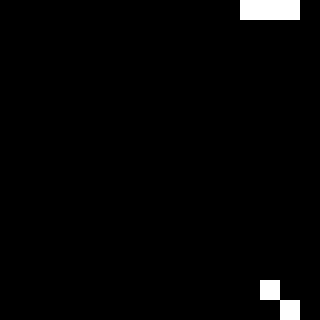
\includegraphics[width=3cm]{pngimages/16-100.png}
\caption{16x16 images.}
\end{figure}

\begin{figure}[H]
\centering
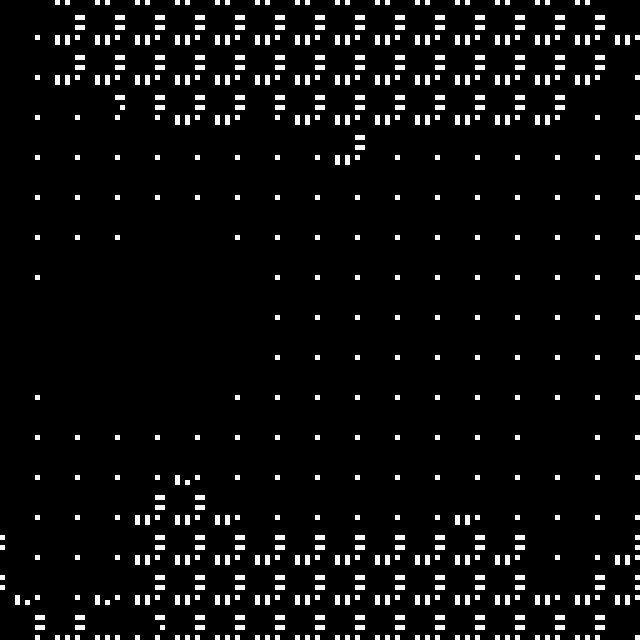
\includegraphics[width=3cm]{pngimages/128-1.png}
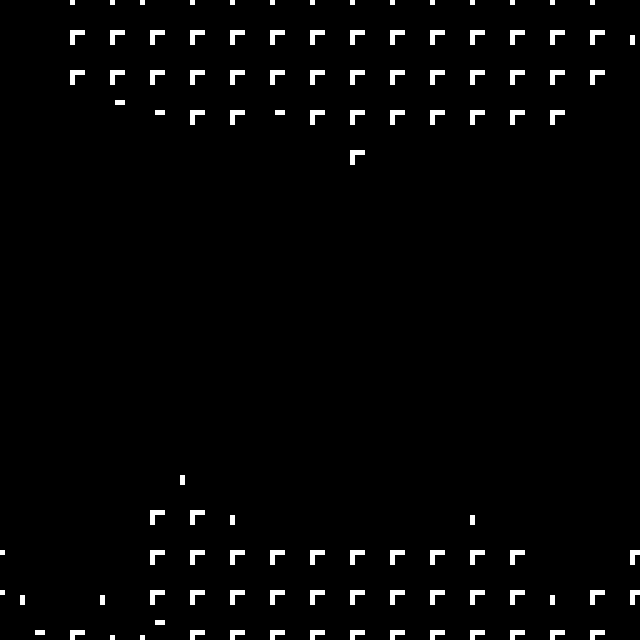
\includegraphics[width=3cm]{pngimages/128-2.png}
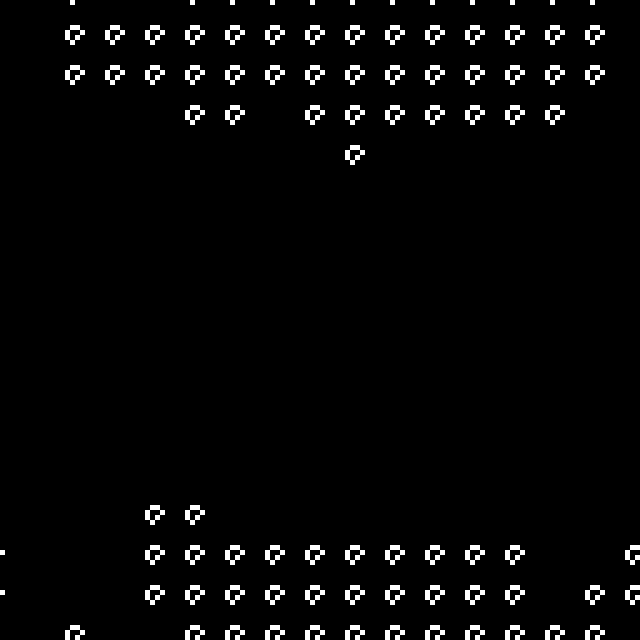
\includegraphics[width=3cm]{pngimages/128-100.png}
\caption{128x128 images.}
\end{figure}

\begin{figure}[H]
\centering
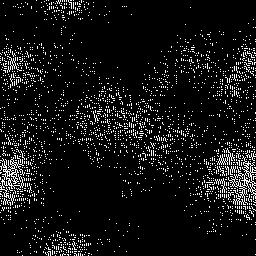
\includegraphics[width=3cm]{pngimages/256-1.png}
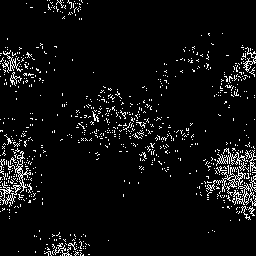
\includegraphics[width=3cm]{pngimages/256-2.png}
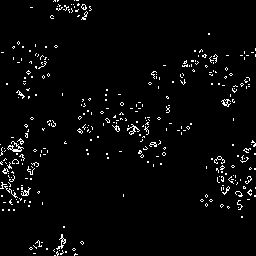
\includegraphics[width=3cm]{pngimages/256-100.png}
\caption{256x256 images.}
\end{figure}

\begin{figure}[H]
\centering
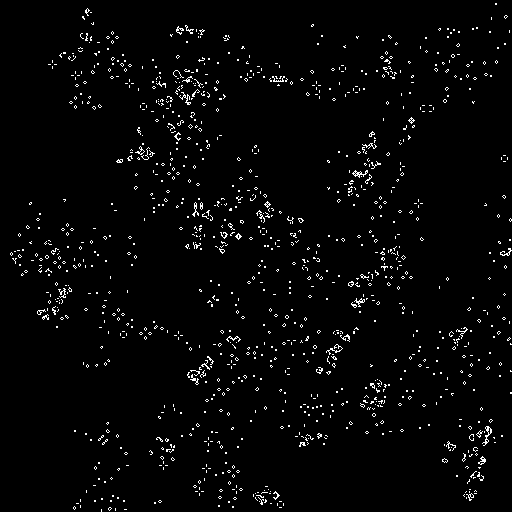
\includegraphics[width=3cm]{pngimages/512-1.png}
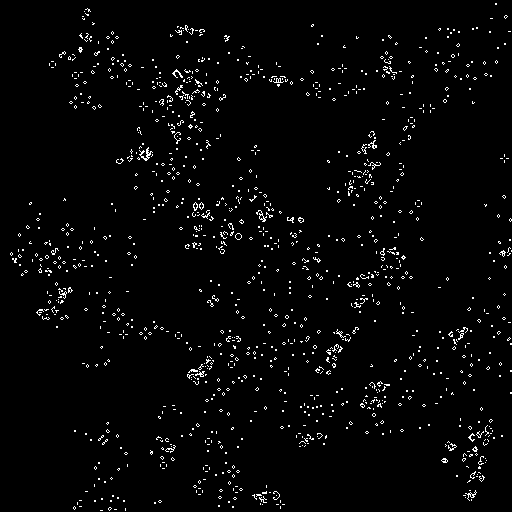
\includegraphics[width=3cm]{pngimages/512-2.png}
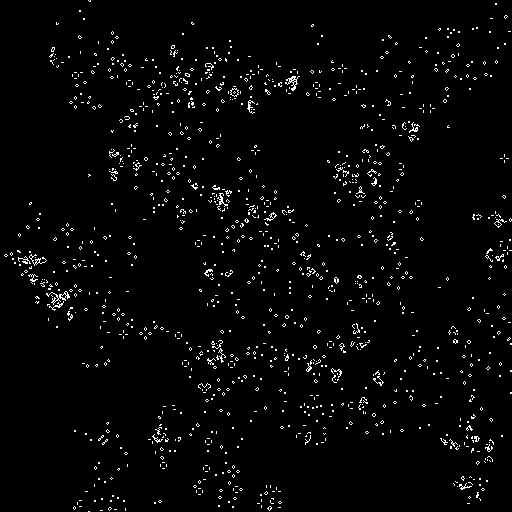
\includegraphics[width=3cm]{pngimages/512-100.png}
\caption{512x512 images.}
\end{figure}

\begin{figure}[H]
\centering

\includegraphics[width=3cm]{pngimages/1024-1.png}
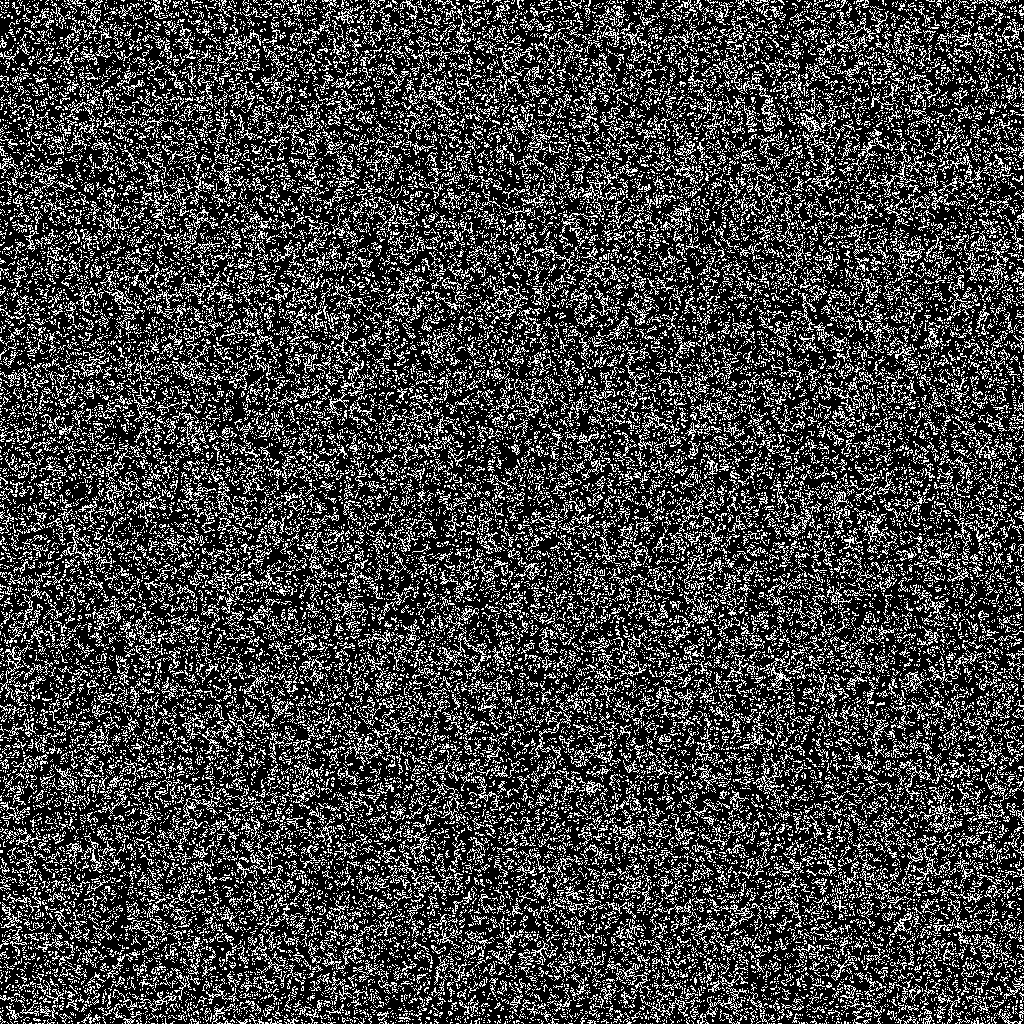
\includegraphics[width=3cm]{pngimages/1024-2.png}

\includegraphics[width=3cm]{pngimages/1024-100.png}
\caption{1024x1024 images.}
\end{figure}

\begin{figure}[H]
\centering

\includegraphics[width=3cm]{pngimages/1264-1.png}

\includegraphics[width=3cm]{pngimages/1264-2.png}

\includegraphics[width=3cm]{pngimages/1264-100.png}
\caption{1264x1264 images.}
\end{figure}

\end{multicols}

\begin{figure}[H]
\centering
\includegraphics[width=3cm]{pngimages/64-0.png}
\includegraphics[width=3cm]{pngimages/64-1.png}
\includegraphics[width=3cm]{pngimages/64-2.png}
\includegraphics[width=3cm]{pngimages/64-3.png}
\includegraphics[width=3cm]{pngimages/64-100.png}
\includegraphics[width=3cm]{pngimages/64-1000.png}
\caption{64x64 image after 0, 1, 2, 3, 100, and 1000 iterations respectively.}
\end{figure}

\begin{center}
\begin{tabular}{ | l | l | l | l | l |}
\hline
   & 1 & 2 & 4 & 8 \\ \hline
16x16 & 0.27 & 0.16 & 0.11 & 0.10 \\ \hline
64x64 & 3.50 & 1.82 & 1.00 & 0.81 \\ \hline
128x128 & 13.40 & 6.81 & 3.54 & 2.83 \\ \hline
256x256 & 52.48 & 26.76 & 13.76 & 11.09 \\ \hline
512x512 & 212.43 & 107.74 & 55.50 & 43.65 \\ \hline
1024x1024 & 849.73 & 431.77 & 220.34 & 174.81 \\ \hline
1264x1264 & 1408.64 & 717.47 & 370.84 & 294.24 \\ \hline
\end{tabular}

\vspace{5mm}

Time taken for the image size specified on the left column \\
to be processed by the number of workers specified on the top row.

\end{center}

\newpage

\begin{figure}[H]
\centering
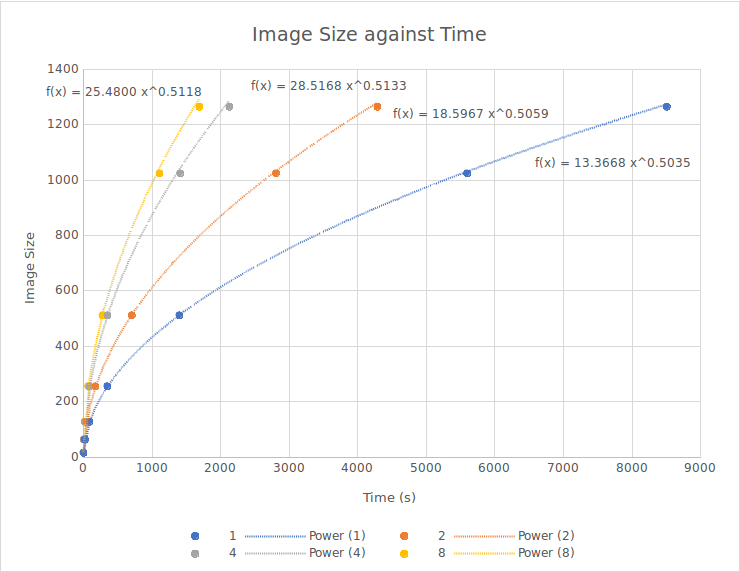
\includegraphics[width=15cm]{ImgvsTime(BeforePow).png}
\caption{Image Size against Time.}
\end{figure}

\begin{figure}[H]
\centering
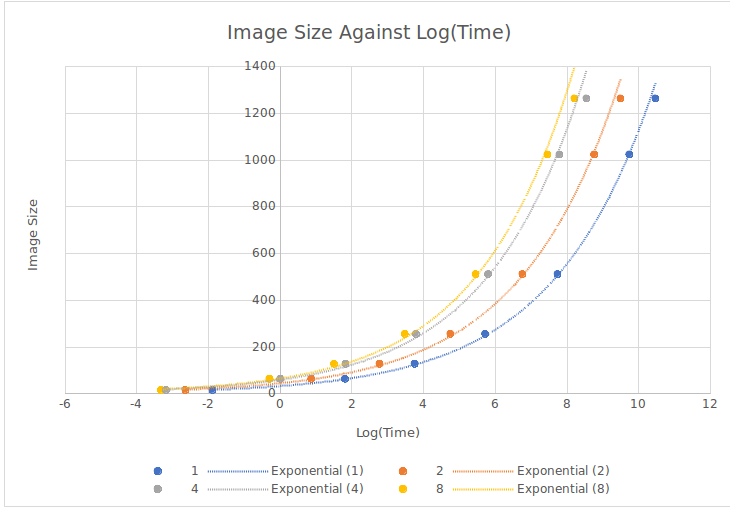
\includegraphics[width=15cm]{ImvsLog(Time)(BeforePow).png}
\caption{Image Size Against Log(Time).}
\end{figure}

\newpage

\newgeometry{margin=2cm}

\begin{multicols}{2}

% Create a new section.
\section{Critical Analysis}
The maximum size our system can process is 1264x1264. Our system can process these large
images quickly, for example our program processes a 1264x1264 image in ~2.9 seconds. Our system
also does well at processing small images, processing 100 iterations of a 16x16 image in 0.10
seconds.

\vspace{3mm}

Looking at the table at the bottom of page 2 shows the time taken for
100 iterations of the Game-of-Life to be processed using different numbers of workers. Initially,
when looking at our table, we noticed that there seemed to be diminishing returns, especially when
increasing from 4 workers to 8 workers. For example, when processing 100 iterations of a 512x512
image, there is a 49.3\% decrease in time taken when increasing from 1 to 2 workers. Similarly,
there is a 48.5\% decrease in time when increasing from 2 to 4 workers. However, when increasing
from 4 to 8 workers, there was only a 21.3\% decrease in time taken.

\vspace{3mm}

This will be a new paragraph.


\vspace{3mm}

We noticed that reading and writing images was very slow initially. We sped this up slightly by
sending a 'packed' array to the distributer instead of an array representing each cell by a byte.
This meant that we were sending a set of values that was 1/8th the size of the set of values that
was originally being sent. However, reading and writing is still extremely slow. If we had
more time for improving the system, perhaps this could be improved by reading in multiple lines
from the file at a time.



% End the two column formatting.
\end{multicols}

% End the document.
\end{document}
